%
% Project Report
%
%
%

%
% Use the standard article template.
%
\documentclass[twoside,11pt]{article}
\usepackage{amsfonts,amsthm,fullpage}
\usepackage{amsmath}
\usepackage{amssymb}
\usepackage{listings}
\usepackage{bm}
% The geometry package allows for easy page formatting.
\usepackage{geometry}
\geometry{letterpaper}
% Load up special logo commands.
\usepackage{doc}
% Package for formatting URLs.
\usepackage{url}
% Packages and definitions for graphics files.
\usepackage{graphicx}
\graphicspath{ {graph/} }
\usepackage{epstopdf}
\usepackage{multirow}
\usepackage{booktabs}
\usepackage{float}
\DeclareGraphicsRule{.tif}{png}{.png}{`convert #1 `dirname #1`/`basename #1 .tif`.png}

%
% Set the title, author, and date.
%
\title{TSP - Comparison of Stochastic Local Search , Heuristic and Exact Algorithm}
\author{Ajay DSouza}
\date{\today}

%
% The document proper.
%
\begin{document}

% Add the title section.
\maketitle

% Add an abstract.
\abstract{
This is a discussion of solving a Traveling Salesman Problem solution using a variety of algorithms. \texttt{MST-Approx, Farthest Insertion, Local Search with 2Opt Exchange with Simulated Annealing,  Local Search with 2Opt Exchange with Simulated Annealing with dynamic neighborhood, Local Search with 2Opt Exchange with iterative search,  Local Search with 2Opt Exchange with random walk , each local search implementation can be executed with different neighborhoods configurations} 
}

% Add various lists on new pages.
\pagebreak
\tableofcontents

\pagebreak
\listoffigures

\pagebreak
\listoftables

% Start the paper on a new page.
\pagebreak

%
% Body text.
%
\section{Introduction}
\label{introduction}
We are provided with sets of nodes where costs between nodes are computed as Euclidean distances or Geographical distances as the case may be. The goal is to explore and compare the different methods of finding the lowest cost Hamiltonian Cycle for the graph and solve the TSP Problem for that graph. I have implemented and executed the following algorithms. The algorithms are implemented as first improvement algorithms.
\begin{enumerate}
\item
Heuristic based algorithm  MST Approx with a guaranteed approximation bound of 2
\item
Heuristic based algorithm Farthest Search which does not have a approximation bound but performs with accuracy in the range of $10-15\%$
\item
A Local Search algorithm with 2 Opt exchange and simulated annealing and a dynamic selection of neighborhood which reduces n size  as the annealing temperature cools
\item
A Local Search algorithm with 2 Opt exchange and simulated annealing with an an option of choosing any K or K all for the neighborhood
\item
A Local Search algorithm with 2 Opt exchange and iterative search through the whole neighborhood
\item
A Local Search algorithm with 2 Opt exchange and random walk in the neighborhood with option for any K or K all for the neighborhood
\item
A branch and bound algorithm using MST as the lower bound
\end{enumerate} 



\section{Problem Definition}
Implement some varieties of Local Search algorithms for the 6 data sets of traveling sales man (TSP) problems. The Local Search algorithms start from a approximate candidate solution and then search the neighborhood to seek to further optimize the candidate solution. The approximate candidate solutions can be generated from one the many heuristic methods available. Some of them have approximation guarantee and some do not. I decided to implement one algorithm of each variety. I implemented the MST Approximation algorithm which has a approximation $p(n)$ of $2$. I also implemented the Farthest Insertion heuristic algorithm which gives good performance in the range of  $10-15\%$ in practice but does not have a proven approximation guarantee.

\section{Related Work}
There has been a lot of experimental work being published on the Local Search improvement methods for solving TSP problems. Local search is empirical by nature. The research suggests that for best results it is required to experiment with Local Search algorithms using the stochastic process of randomization the parameters for Local Search algorithms. This is known in practice to help at arriving at the optimum values for the parameters of the particular Local Search Algorithm being considered in a particular environment. In our case the parameters for local search that need to be tuned are the neighborhood size, the exchange method, the choice of neighbors, the threshold for acceptance of bad trades during simulated annealing, the run time, the start temperature, the cooling rate, thresholds for reheating and restarting etc. Well chosen parameters will give better Local Search results.

\section{Algorithms}
I have implemented five algorithms in three different families of algorithms. The MST approximation algorithm with a guaranteed bound, the Farthest Insertion approximation algorithm with no guaranteed bound and three different types of Local Search algorithms which seeks the improve the TSP obtained by the Furthest Insertion approximation. The Local Search Algorithms implemented uses 2Opt exchange method to trade two edges for possibly 2 new edges. I have implemented flavors of local search algorithms with both random walk style selection of edges to exchange as well as the systematic iterative search of the neighborhood for better edges. Local search allows for trades that get it closer to the optimum. But with Simulated Annealing we allowing for bad trades based based on random probability with an intention to not get stuck in local minimums. The probability for bad trades lowers as the annealing temperature cools. The new edges are searched in the neighborhood specified. The default neighborhood is K=5. A flavor of the local search with simulated annealing takes a dynamic neighborhood, a neighborhood that reduces in size as the annealing temperature cools. This is to allow for search in the local optima area after wider searches to explore the whole search space at higher temperatures.

\subsection{Implementation}
The following is the pseudo code for the algorithms implemented. 
\subsubsection{MST Approx Algorithm}
MST Approx Algorithm. Prim is preferred over Kruskal as this is a TSP problem with dense edges. The MST Approx algorithm is implemented using Prims algorithm for generating the MST using Fibonacci heap and runs in $\mathbf{O}(m\log n)$.
\lstset{language=java, basicstyle=\footnotesize,frame=single,keepspaces=false,tabsize=1,escapeinside={\%*}{*)}}
\begin{lstlisting}
/*
 * Invoke the approx mst to get the TSP
 */
LinkedList mstApprox(File fileNameWithPath) 

1 read the file and build the cost table
2.record start time 
3. Invoke Prims algorithm with random seed to get the MST
	3.1 Use the seed passed to pick the the random start node in 
	Prims Algorithms so the same random seed gives the same MST 
	each time
	3.2 Use Fibonaci heap for best performance when choosing the
	lowest priority edge across the cut each time 
	3.3 Loop over each edge 
	3.4 every step picking the lowest cost 
	edge from the nodes that are not in MST to the nodes that are
	in MST 
	3.5 Add that edge to the MST and update priority for the 
	new edges that are now across he cut from the new node added 
4. Do a depth first traveral on the MST returned in 3
5. Select the pre order sequence of vertices and save them in a 
	linked list
	5.1 Use a LIFO stack to traverse the MST depth first
6. This linked list of preorder sequence of vertieces from MST
is the TSP solution
7. Add the first node back again at the end of the linked list to 
complete the TSP cycle
8. Record Finish time
9. Record results
\end{lstlisting}
\subsubsection{Farthest Insertion Heuristic Approximation}
Psuedo code for the implemented Farthest Insertion Algorithm.  The Furthest Insertion algorithms is implemented using Fibonacci heaps to pick the max distance vertex and runs in the order of $\mathbf{O}(n^2)$.
\lstset{language=java, basicstyle=\footnotesize,frame=none,keepspaces=false,tabsize=1,escapeinside={\%*}{*)}}
\begin{lstlisting}
/*
 * Invoke the greedy furthest insertion heuristic to get the TSP
 */
LinkedList heurFurthestInsertion(File fileNameWithPath) 
	
1 read the file and build the cost table
2.record start time 
3. Invoke the Farthest Insertion Algorithm , with a random seed to
 generate TSP
	3.1  Use the seed passed to pick the the random start node in 
	Prims Algorithms so the same random seed gives the same MST 
	each time
	3.2 Use Fibonaci heap for priority Q, for best performance
	when choosing the lowest priority edge across the cut each time 
	3.2 Add the randomly picked start node to the TSP linkedList
	3.4 Add all vertices on edges from that node to the Priority Q, 
		by negating their costs
	3.3 Next dequeue from PQ the min priority vertex (max cost edge
	as PQ stores based on negative cost) from that start node to 
	any other vertex
	3.4 Add the new vertex to the TSP
	3.5  Add all vertices on edges which are not yet in TSP,from that 
	newly added vertex to the Priority Q, by negating their costs
	3.6  Loop till we cover all vertices
		3.6.1 dequeue from PQ the min priority vertex(k)(max 
		cost edge as PQ stores based on negative cost)
		from that start node to any other vertex
		3.6.2 Find an edge (i,j), where gives the min cost 
		for inserting the dequeued vertex l between as 
		min (c_ik+c_jk-c_ij)
		3.6.3 Insert the vertex k between vertices( i,j) in
		 the TSP
		3.6.4 Next, add all vertices on edges which are not
		 yet in TSP, from that inserted vertex  k to the 
		 Priority Q, by negating their costs
	3.7 Add the first node back again at the end of the linked list 
	to complete the TSP cycle
8. Record finish time 
9. Record Results 	
\end{lstlisting}
\subsubsection{MST Approx}
Psuedo code for the Local Search with neighborhood 2Opt exchange with simulated annealing.
\lstset{language=java, basicstyle=\footnotesize,frame=none,keepspaces=false,tabsize=1,escapeinside={\%*}{*)}}
\begin{lstlisting}
/*
 * Invoke the local search simulated annealing algorithm with 2 opt
 */
LinkedList localSearchSimulatedAnnealing(File fileNameWithPath) 
		
		
1 read the file and build the cost table
2. Invoke the Farthest cost algorithm discussed above to get a candidate 
TSP solution as current TSP
3. Record this as the bestTsp so far with the best cost
4. record base start time
5. Seed the random number generator
6. Record the bestTsp
   7. Initialize initialising parameters
   7.1 coolingRate
   7.2 Start tempreature
   7.3 Random acceptance probability threshold for bad trades
8. loop ( tempreate has not cooled  )
8.1 If we have reached the cutoff time , then break loop
8.2 record start time for cycle
8.3 Create a newTsp from currentTsp by doing the following for 
	neighborhood 2Opt exchange
	8.3.1 Randomly choose a edge in the current TSP (v2,v2-1)
	8.3.2 Randomly choose a different edge (v3+1,v3) where v3 is within the
	(k=5) nearest nighbors of v2 and is not adjacent to v2
	8.3.3 Now in the TSP remove the links for edges (v2,v2-1) and (v3+1,v3)
	and swap them with these links for new edges as follows
	8.3.4 In the TSP linkedList connect v2-1 to v3
	8.3.5 In the TSP linkedList connect v2 to v4
	8.3.6 save the modified TSP as newTsp 
8.4 If cost of the newTSP is better then the cost of the currentTSP, 
	8.4.1 replace the currentTSP with the newTSP
8.5 If the cost of the newTSP is more then the currentTSP, then 
	8.5.1 Check of the probability calculated as follows is better then a 
	randomly chosen probability
	(1/e^( newTspCost - currentTSPCost )/ T <- cooling tempreature )
	8.5.2 If it is better then replace currentTSP with the worse newTSP
8.6 If cost of currentTSP is lower then bestTSP cost, then replace bestTSP
	with current TSP
8.7 record end of current cycle
8.8 record trace results
9. Record finish time 
10. Record Results 	
\end{lstlisting}

\subsection{Collateral}
\begin{enumerate}
\item
The file README-dl-ajdsouza31.txt gives the details of executing the file, the following is an overview
\item
The project is implemented in Project.class. This is the top level program.
\item
All the class files are compiled on windows 8, 64 bit with Intel Core $I7 2.5 Ghz$ processor and $16GB$ of memory box, and are archived in Project.jar
\item
To execute the project, 
\begin{lstlisting}
java -cp <classpath if extracted the class files from jar or the path 
      to the jar file>Project.jar Project
<file_name_with_full_absolute_path> <cutofftime_seconds>
<method[bnb|mstapprox|heur_furthest_ins|ls_2opt_sa_dyn|ls_2opt_iter|ls_2opt_k5|ls_2opt_kall|ls_2opt_sa_k5|ls_2opt_sa_kall]> 
[<random_seed_for_random_search_algorithms>] [<runId-for local search algorithms>
[<K_for_neighborhood for local search>
\end{lstlisting}
\item
Here are some examples of execution
\begin{lstlisting}

echo "MST Approx"
java -cp Project.jar Project C:\\wk\\project\\DATA\\burma14.tsp 100 mstapprox


echo "Heuristic Furthest Insertion"
java -cp Project.jar Project C:\\wk\\project\\DATA\\burma14.tsp 100 heur_furthest_ins


echo "Local Search - 2opt  with k5 neighborhood "
java -cp Project.jar Project C:\\wk\\project\\DATA\\burma14.tsp 100 ls_2opt_k5 5 1

echo "Local Search - 2opt with with iterative search"
java -cp Project.jar Project C:\\wk\\project\\DATA\\burma14.tsp 100 ls_2opt_iter 5 1


echo "Local Search - 2opt with Simulated Annealing with dynamic neighborhood "
java -cp Project.jar Project C:\\wk\\project\\DATA\\burma14.tsp 100 ls_2opt_sa_dyn 5 1

echo "Local Search - 2opt with Simulated Annealing with k5 neighborhood "
java -cp Project.jar Project C:\\wk\\project\\DATA\\burma14.tsp 100 ls_2opt_sa_k5 5 1


echo "Local Search - 2opt  with full neighborhood "
java -cp Project.jar Project C:\\wk\\project\\DATA\\burma14.tsp 100 ls_2opt_kall 5 1


echo "Local Search - 2opt with Simulated Annealing with full neighborhood "
java -cp Project.jar Project C:\\wk\\project\\DATA\\burma14.tsp 100 ls_2opt_sa_kall 5 1


\end{lstlisting}
\item
The output files are generated in the SAME directory from where you are executing the program.
\end{enumerate}


\section{Empirical evaluation}
The following are the tabulated results for four of the varieties of algorithms that I implemented. The Farthest Insertion heuristic algorithm consistently gives results which are much better then the MST Approx algorithm. This is of interest as there is no approximation bound on the Farthest Insertion algorithm, while the MST Approximation algorithm has a approximation ratio $p(n)$ of 2. The run times of both the heuristic approximation algorithms where the same in sub seconds for all the data sets provided. 
For local search algorithms I have implemented a 2Opt exchange in a variety of flavors. You could execute the 2Opt local search either as an systematic iterative search in the whole neighborhood, or as a random walk where candidate edges for exchange are chosen in stochastic fashion. For each local search you can specify the neighborhood size to search in. The neighborhood size is specified as a command line option. The default neighborhood size for local search is K=5 and remains fixed throughout the search process. However there is an implementation of simulated annealing where the neighborhood is dynamic and gets reduced as the annealing temperature cools. The neighborhood starts from a size of $N/2$ and gets reduced gradually by a rate of $.99$ as the temperature cools.  I have also implemented the branch and bound algorithm, however it is not advertised as the java data structures used quickly run out of memory when exploring the path tree. Branch and bound for the data sets does not seem to be a very efficient algorithm.

I have experimented with arange of different options for the Local Search algorithms such as various start temperatures, cooling rate, neighborhood choice, neighborhood selection, restarting from a earlier better solution when stuck in plateau cycles, reheating when simulated annealing is stuck in a local optima. Local Search algorithm with Neighborhood 2Opt and simulated annealing requires substantial run time so that the parameters can be fine tuned for even better execution.  I noticed that local search with simulated annealing and dynamic neighborhood gave good results for the smaller datasets of burma14,ulysses16,berlin52 reaching optimum in reasonable time. I have posted the best results in the document. However for larger datasets of ch150,gr202 similar performance could not be achieved. This suggests that the annealing parameters need to be tuned better for better results. Local Search with simulated annealing requires a very gradual decrement in annealing tempreature in each cycle and with it longer run times to reach closer to the optimum for larger data sets.

\subsection{Comprehensive Table}
\item
The comprehensive table of results for the four of the different flavors of algorithms implemented. As can be seen the Local Search improves on the results of the Farthest Insertion algorithm for most cases. However this improvement is very slight and further improvement can be achieved with better tuned parameters and longer run times. The improvement that the Local Search does over the results of the Furthest Insertion Algorithm are very slow and very gradual. In every case the Furthest Insertion heuristic algorithm betters the MST Approx algorithm very decisively. They both have similar run times and execute in subs seconds. In the case of $burma14.tsp,ulysses16.tsp,berlin52.tsp$, the best results of the Local search reach the optimum. The values plotted for the Local Search algorithm in the table are the average results over several runs. The Local Search I is the Local Search with 2Opt with simulated annealing with dynamic neighborhood and Local Search II is the Local Search with 2Opt exchange with random walk with a K=5 neighborhood. These two local searches gave the best results among the different flavors of algorithms that I experimented on.
\item
The tabulated results are the experimental results for all five algorithms on all six datasets. Time is in seconds, and Relative error (RelErr) is computed as $(AlgPathLength - OPTPathLength)/ OPTPathLength)$. Bold values for RelErr highlight the closest algorithm to the optimum for a given dataset. 
\begin{table*}[!htbp]
\caption{Algorithm Results Table}
\tabcolsep=0.11cm
\begin{tabular}{lccccccccccccccc}
\toprule
\multirow{2}[3]{*}{Dataset} & \multicolumn{3}{c}{Local Search I} & \multicolumn{3}{c}{MST Approx}  & \multicolumn{3}{c}{Farthest Insertion}  & \multicolumn{3}{c}{LS Search II}& \multicolumn{3}{c}{Local Search III}\\
\cmidrule(lr){2-4} \cmidrule(lr){5-7} \cmidrule(lr){8-10} \cmidrule(lr){11-13} \cmidrule(lr){14-16}
 & Time & Length & RelErr & Time & Length & RelErr & Time & Length & RelErr & Time & Length & RelErr & Time & Length & RelErr\\
\midrule
burma14 & 0.00 & 3474 & \bf 0.0460 & 0.00 & 4125 & 0.2400 & 0.00 & 3487 & 0.0500 & 0.01 & 3474 & \bf 0.0456 & - & - & - \\
ulysses16 & 0.01 & 7065 & \bf 0.0317 & 0.01 & 7604 & 0.1050 & 0.01 & 7064 & \bf 0.0300 & 0.01 & 7054 & \bf 0.0300 & - & - & - \\
berlin52  & 0.01 & 8123 & \bf 0.0760 & 0.01 & 9964 & 0.3200 & 0.01 & 8222 & 0.0900 & 0.01 & 8569 & 0.1400 & - & - & - \\
kroA100  & 0.01 & 24272 & \bf 0.1400 & 0.01 & 29256 & 0.3700 & 0.01 & 24312 & \bf 0.1400 & 0.02 & 24492 & \bf 0.1508 & - & - & - \\
ch150  & 0.03 &  7115 & \bf 0.1516 & 0.03 & 9323 & 0.4250 & 0.02 & 7490 & \bf 0.1500 & 0.05 & 7504 & \bf 0.1493 & - & - & - \\
gr202 & 0.05 &  45065 & 0.1222 & 0.06 & 53158 & 0.3250 & 0.05 & 44654 & \bf 0.1100 & 0.06 & 44966 & \bf 0.1196 & - & - & - \\
\bottomrule
\end{tabular}
\end{table*}

\subsection{Qualified Runtime for various solution qualities (QRTDs)}
The Qualified Run Time Distribution for the two largest sets provided ch150 and gr202 can be seen in the following figures. These QRTD plots are for the Local Search with Simulated Annealing with Dynamic Neighborhood method which has given the best results in my implementation.
\begin{figure}[!htbp]
\centering
\caption{QRTD for ch150with Local Search with Simulated Annealing with Dynamic Neighborhood}
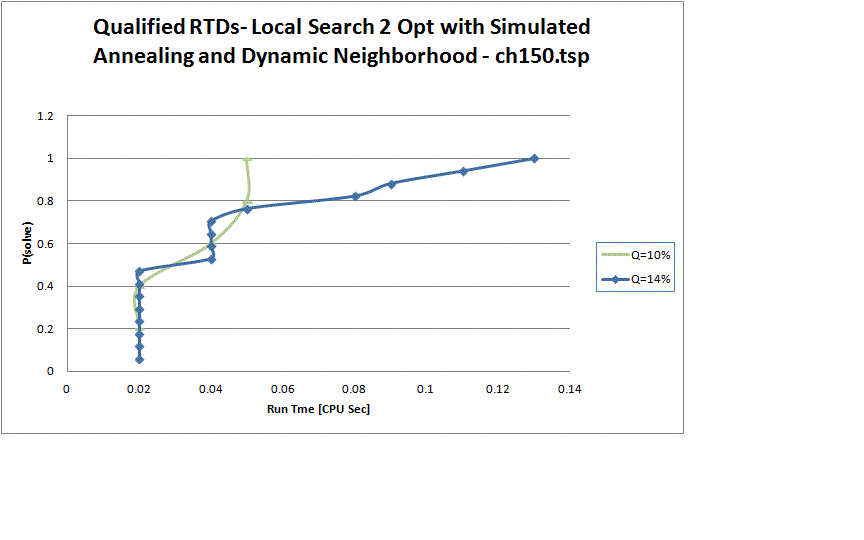
\includegraphics[scale=.85]{images/qrtd_dyn_ch150}
\end{figure}
\begin{figure}[!htbp]
\centering
\caption{QRTD for ch150with Local Search with Simulated Annealing with Dynamic Neighborhood}
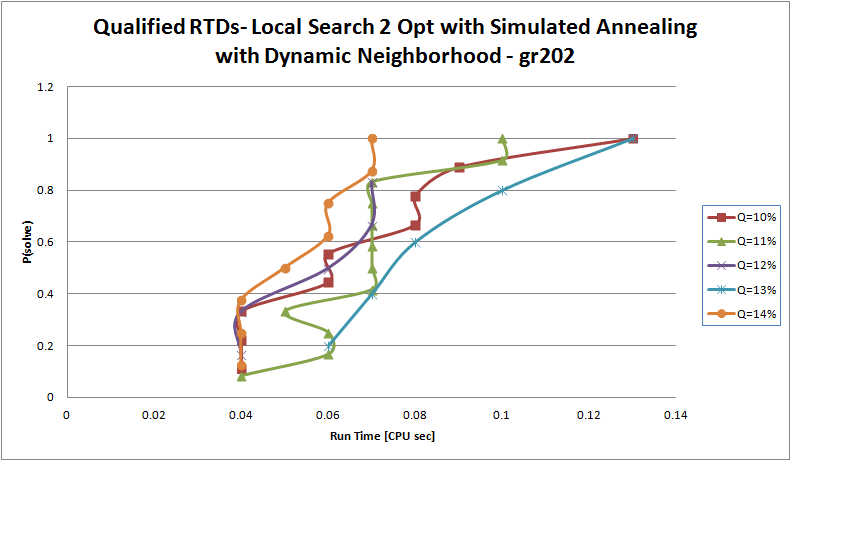
\includegraphics[scale=.85]{images/qrtd_dyn_gr202}
\end{figure}

 
\subsection{Solution Quality Distributions for various run-times (SQDs)}
The Solution Quality Distribution  for the two largest sets provided ch150 and gr202 can be seen in the following figures. These SQD plots are for the Local Search with Simulated Annealing with Dynamic Neighborhood method which has given the best results in my implementation.
\begin{figure}[!htbp]
\centering
\caption{SQD for ch150.tsp with Local Search with Simulated Annealing with Dynamic Neighborhood}
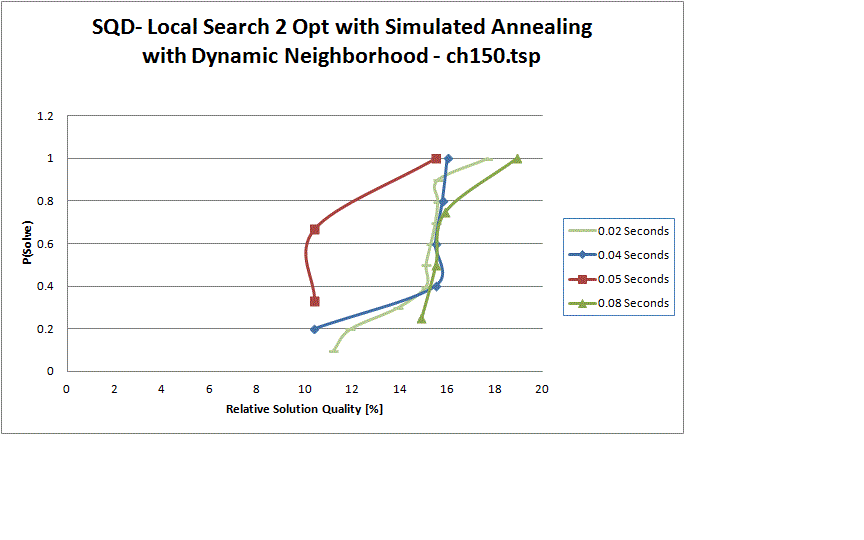
\includegraphics[scale=.9]{images/sqd_dyn_ch150}
\end{figure}
\begin{figure}[!htbp]
\centering
\caption{SQD for gr202.tsp with Local Search with Simulated Annealing with Dynamic Neighborhood}
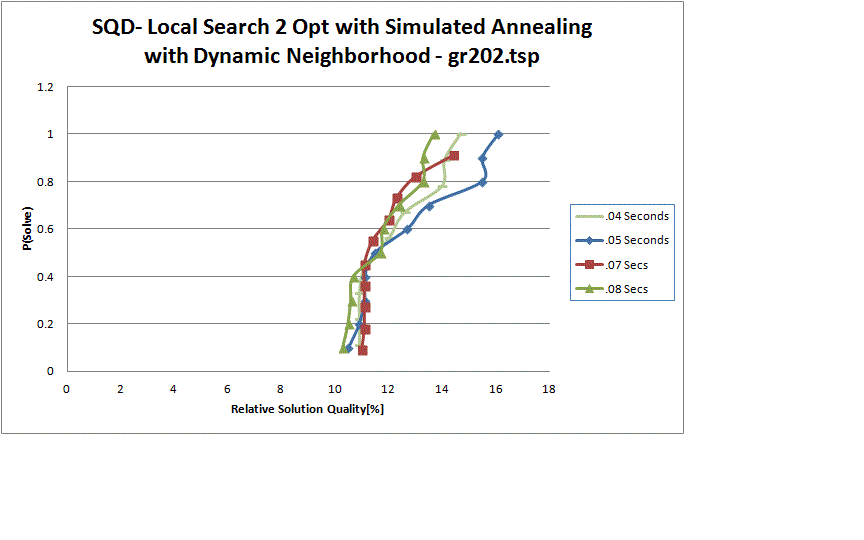
\includegraphics[scale=.9]{images/sqd_dyn_gr202}
\end{figure}
\subsection{Box plots for running times}
The following is the box plot for the Local Search 2Opt Exchange Random Walk, and  Local Search 2Opt Exchange with Simulated Annealing. Both are with a neighborhood of K 5.
\begin{figure}[!htbp]
\centering
\caption{Box Plot for the Local Search 2Opt Exchange Random Walk, and  Local Search 2Opt Exchange with Simulated Annealing with K 5 neighborhood}
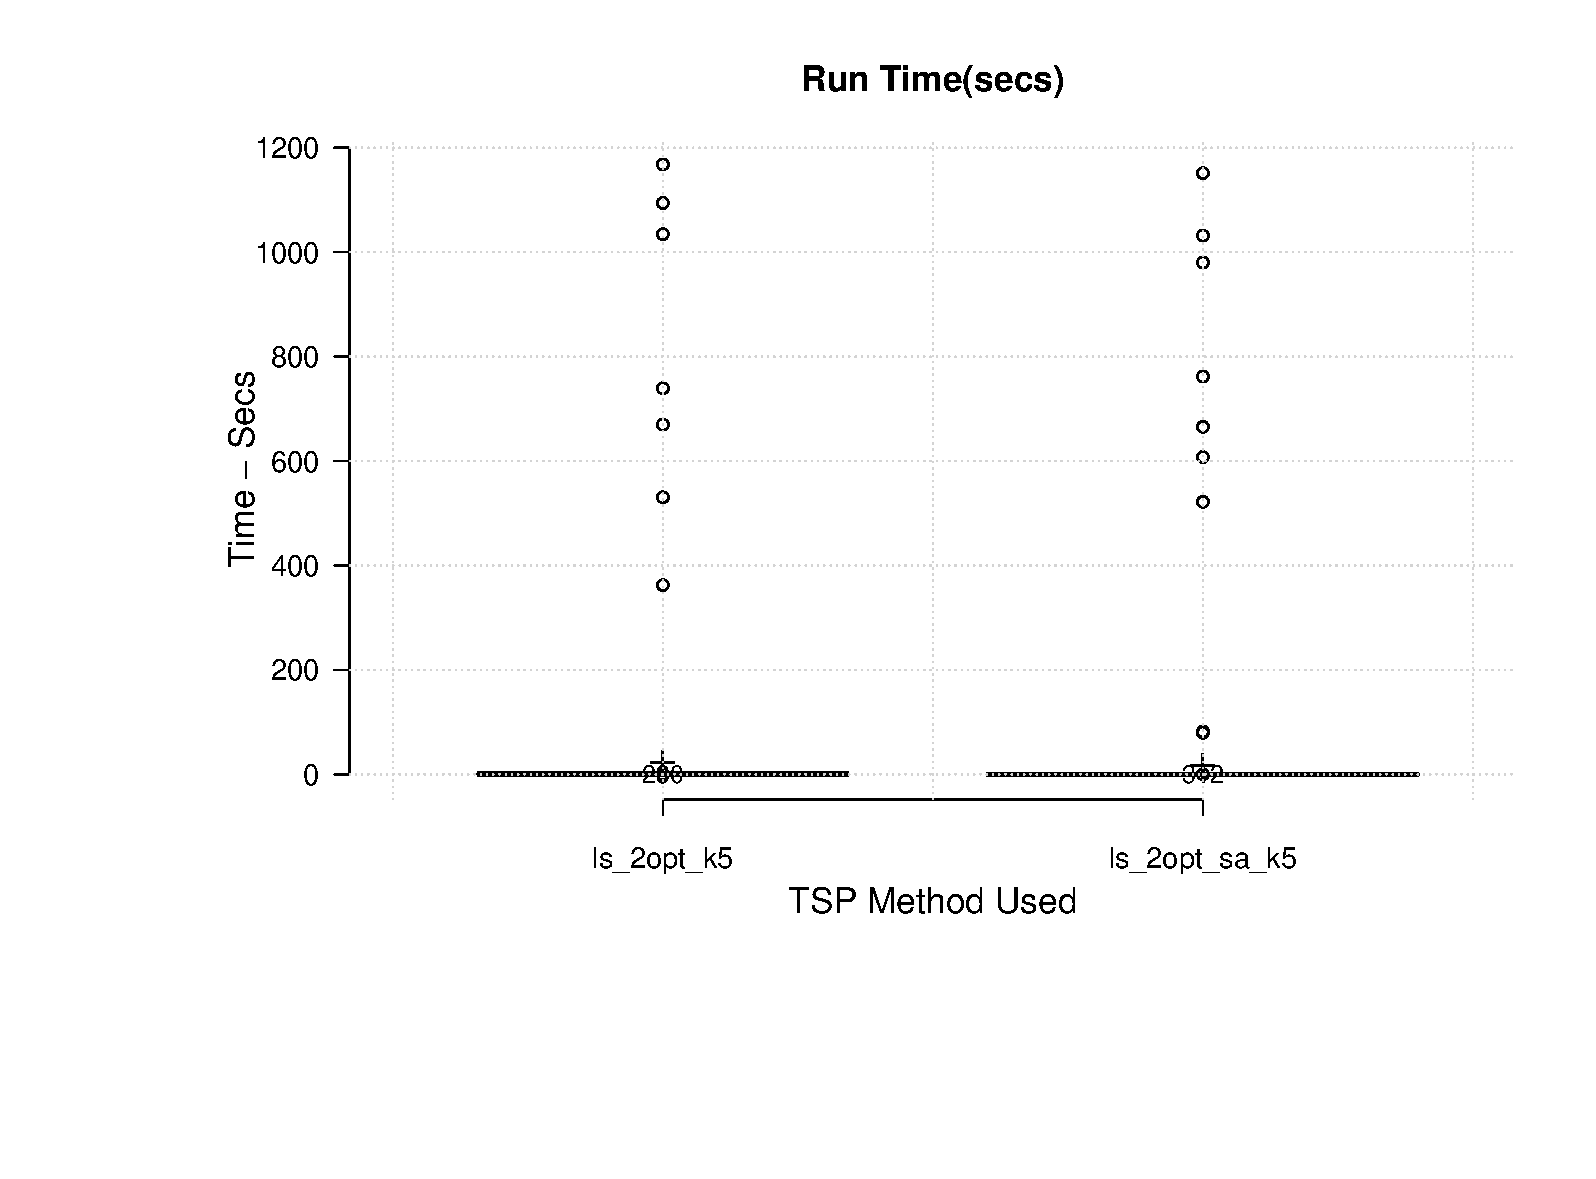
\includegraphics[scale=.7]{images/boxplot}
\end{figure}
 
\section{Issues faced}
\begin{enumerate}
\item
Local Search algorithm needs experimenting with different parameters which determine the nature of local search. Local Search requires very long run times on larger data sets and improvement may not be seen for considerable periods of time. 
\item
For the branch and bound algorithm if the lower bound is not very tight or if we have many paths with lower bounds in the same range, we could end up exploring a lot of paths affecting performance and resource consumption on the machine.
\end{enumerate}


\section{Discussion}
For lower sizes of data the Local Search with Simulated Annealing with 2Opt exchange and a dynamic neighborhood was able to reach the optimum. However for the larger data sets of ch150 and gr202, the very same algorithm was stuck in local optima and able to reach just close to $10\%$ of the optimum. It appears that for larger data sets one needs to experiment local search algorithms to come up with the right search parameters. With those parameters we need to them run local search for considerably longer periods of time to see improvement. This makes sense as the local search is stochastic and longer run times give a better probability of guessing the right neighbor to trade. The Local search with simulated annealing and dynamic neighborhood algorithm performed the best in my implementation. This algorithm was able to reach the optimum with smaller data sets of $burma14,ulysses16,berlin52$, but for the larger data sets the algorithm gets repeatedly gets stuck for long cycles without any improvement.
I think the local search algorithms can be made to search intelligently by helping them choose the right neighborhood, preventing them from getting into cycles and by helping them to get out of a neighborhood when there is no improvement. Using a taboo list would be helpful in this case to prevent cycles. A more intelligent search for neighbors where we keep track of the best performing neighborhoods and revert back to them when the algorithm is stuch. I tried to use reheating when the simulated annealing algorithm was stagnant for long cycles. The following are the best results I was able to achieve. 
The following table tabulates the best results achieved on each dataset
\begin{table*}[!htbp]
\centering
\caption{Algorithm Best Results Table}
\tabcolsep=0.11cm
\begin{tabular}{lcccr}
\hline
Dataset    & Best Length & RelErr & Time & Algorithm \\
\hline
burma14      & 3323    & \bf 0.0000 & 0.00 &  ls\_2opt\_sa\_dyn     \\
ulysses16    & 6859    & \bf 0.0000 & 0.03 &  ls\_2opt\_sa\_dyn     \\
berlin52     & 7542    & \bf 0.0000 & 0.01 &  ls\_2opt\_sa\_dyn     \\
kroA100     & 22413    & \bf 0.0500 & 0.02 &  ls\_2opt\_k5     \\
ch150     & 7208    & \bf 0.1000 & 0.04 &  ls\_2opt\_k5     \\
gr202     & 44281    & \bf 0.1000 & 0.07 &  ls\_2opt\_sa\_k5     \\
\hline
\end{tabular}
\end{table*}

\item
The details of the paramaters used for these results are as below
\begin{verbatim}
burma14 - ls_2opt_sa_dyn - (random seed = 3502400 ) - (cutofftime-7200secs)
Best Cost : 3323 
Relative error: 0.00
CpuTime : 0
Path:
13,3,11,8,10,6,1,2,14,4,7,5,9,12,13

berlin52 - ls_2opt_sa_dyn - (random seed = 6288377 ) - (cutofftime-7200secs)
Best Cost : 7542 
Relative error: 0.00
Cpu Time : 0.01
Path 45,33,41,19,22,10,48,6,4,17,26,35,13,3,52,15,43,34,7,2,23,14,24,21,44,12,38,8,32,36,40,30,50,20,25,27,9,46,49,39,47,28,16,29,11,42,31,51,18,37,1,5,45

ulysses16 - ls_2opt_sa_dyn -  (random seed = 3798284 ) - (cutofftime-7200secs)
Best Cost: 6859 
Relative Error : 0.00 
CpuTime: 0.03 
Path:7,6,14,12,4,16,13,10,3,11,8,5,15,2,1,9,7

kroA100 - ls_2opt_k5 - (random seed = 4901073 ) - (cutofftime-7200secs)
best cost : 22413 - 
Relative error : 0.05
Cpu Time : 0.02
Path :  3,23,67,87,98,41,18,59,97,100,50,31,75,47,62,57,66,20,17,93,40,61,46,49,86,52,54,26,15,53,96,7,2,45,82,27,10,60,74,48,83,90,63,30,80,5,25,39,68,14,99,65,69,38,44,76,51,36,11,88,72,89,73,13,35,28,85,9,22,33,71,4,29,79,34,55,81,24,43,84,91,94,95,64,37,42,70,32,16,12,19,77,6,1,8,56,78,21,92,58,3


ch150 - ls_2opt_k5 - (random seed = 5813517 ) - (cutofftime-7200secs)
Best Cost: 7208 
Relative Error : 0.10 
CpuTime: 0.04
Path: 17,128,43,16,53,87,59,14,122,38,102,114,6,111,150,99,68,134,82,67,124,143,127,141,44,1,58,19,60,116,22,42,15,119,104,40,144,36,83,56,34,136,105,115,72,54,80,32,89,66,50,65,126,94,28,69,117,103,96,52,78,11,118,97,63,18,88,61,145,39,75,29,7,31,24,47,100,125,73,55,33,86,62,5,146,25,106,130,137,90,57,149,132,84,121,109,129,120,23,41,91,131,10,70,21,108,79,81,27,12,123,92,48,2,45,138,51,110,71,76,140,9,85,74,101,35,98,46,64,148,13,95,30,8,20,133,147,49,26,77,142,112,107,3,4,93,113,37,139,135,17


gr202 - ls_2opt_sa_k5 - (random seed = 4373081 ) - (cutofftime-7200secs)
Best Cost: 44281 
Relative Error : 0.10 
CpuTime: 0.07
Path: 137,145,178,110,127,56,200,42,86,100,120,77,40,154,165,34,181,102,22,31,118,80,180,78,51,107,26,193,65,161,121,29,9,15,36,173,79,94,92,142,89,55,7,3,106,194,18,43,45,99,131,146,68,117,134,141,85,91,27,171,199,122,163,58,149,159,133,82,93,130,152,176,32,116,37,139,151,160,63,186,50,155,174,83,81,35,103,47,172,13,5,157,167,62,10,11,135,14,57,19,153,98,150,113,112,136,183,25,192,88,67,101,179,189,125,23,87,97,66,95,39,108,168,73,53,90,190,109,188,4,143,147,28,59,185,105,21,175,64,148,114,52,76,187,170,119,124,69,111,24,71,17,198,48,16,72,70,191,49,197,166,8,182,202,54,126,201,196,115,96,104,164,33,41,44,12,84,162,75,1,184,169,195,140,158,132,74,138,20,61,144,38,156,46,128,123,30,60,6,129,177,2,137

\end{verbatim}


\section{Conclusion}
\begin{enumerate}
\item
The Farthest Insertion heuristic approximation algorithm consistently gives better results that the MST Approx algorithm. Both the algorithm are not very dissimilar in their run times. While MST Approx has a bound guarantee on its results being not more that twice optimum, the Farthest Insertion algorithm offers no such guarantee. However in practice the Farthest Insertion performs betters the MST Approx consistently with similar run times
\item
The two approximation algorithms explored and implemented here have stochasticity only in the selection of the starting vertex. With the start vertex fixed with take away the stochasticity and fix the start vertex the algorithms repeat the results.
\item
Local Search which are stochastic in nature, with stochasticity in many dimensions. For best local search results it is required to come up with a optimum  set of these stochastic parameters. Getting these optimal parameters for local search is  experimental in nature and requires the local search to be run multiple times with considerable long run times.
\item
If we are using local search to further optimize a good candidate solution from a approximation algorithm, then for larger data sets even a well tuned local search algorithm might need to be run for longer times for them to show any improvement. The probability of local search giving optimizing gets better with longer run times. 
\item
Local Search with 2Opt exchange was tried with different flavors such as systematic iterative and random walk, with varying sizes of neighborhoods as well as dynamic neighborhoods and with simulated annealing with reheating. The Local Search with 2Opt Exchange with dynamic neighborhood $(ls_2opt_sa_dyn)$, which reduces in size as the temperature cools gave the best results on a average. The algorithm reached the optimum for $burma16, ulysses16, berlin52$ datasets, it reached within $5\%$ for the $kroA100$ dataset and within $10\%$ for the largest data sets of $ch150 ,gr202$. This indicates that the annealing parameters of the algorithm need further tuning.
\item
It appears for the $(ls_2opt_sa_dyn)$ could do better on larger datasets if we could reheat the annealing temperature when it is stuck in a unstable state for long cycles. Using a Taboo list would also be an enhancement that would make the search more intelligent along with remembering performances in different neighborhoods so the algorithm could go back to them when stuck.
\item
The branch and bound algorithm appears to work only if we have a very tight lower bound and there is a wide range of variation in the lower bounds on different paths. Else the branch and bound could be a resource hog trying to explore a large part of the $n!$ paths.
\end{enumerate}

% Generate the bibliography.
\bibliography{latex-sample}
\bibliographystyle{unsrt}

\end{document}
